\section{Functional Description}
%----------------------- Functional description ----------------------------
\label{sec:functional_description}

This section provides a detailed description of the internal building blocks of Sesnando.

\begin{itemize}
\item Command Line Arguments (Section \ref{subsec:command_line_arguments}) - presents the arguments that \textit{Sesnando} supports from the command line.
\item Input requirements (Section \ref{subsec:sesnando_input}) - Presents examples of the requirement structure that \textit{Sesnando} supports.
\item Requirement processing (Section \ref{subsec:requirement_processing}) - Presents the compilation of the requirement into a Parse tree and how a XML sample can be obtained by using Debug mode.
\item Grammar Elements (Section \ref{subsec:grammar_elements}) - Presents the installed grammar on \textit{Sesnando} and how requirements should be defined.
\item Signal Mapping (Section \ref{subsec:signal_mapping}) - Presents how Requirement signals are translated into Software signals.
\item Test Generation (Section \ref{subsec:test_generation}) - Presents how \textit{Sesnando} compiles input requirements and how tests are generated on a design level.
\item Signal Manager (Section \ref{subsec:signal_manager}) - Presents the main role of Signal manager on test generation and overview of its user interface.
\item Test Designer (Section \ref{subsec:test_designer}) - Presents the test designer user interface, and how test specifications are visualised with the aid of this module.
\end{itemize}


\subsection{Command Line Arguments}
%----------------------- Command Line Arguments ----------------------------
\label{subsec:command_line_arguments}

At the moment, Sesnando operates as a command line application. The command line arguments can be passed at the application launch, but a configuration file can be set, so that the user can define a set of default parameters avoiding the need to pass the arguments at all times. Default values from the configuration file will be used when omitting these parameters from the command line. The available command line arguments are defined on Table \ref{tab:CLI}.

As \textit{Sesnando} can be executed following a set of parameters from the command line or from a \textit{JSON} configuration, a detailed description of these commands are as follows.

\begin{itemize}
    \item signal\_manager - The address of the remote Signal Manager server, containing the data required to successfully generate test cases. Default port 5001.
    \item input - The location of the input file containing the requirements to be parsed by \textit{Sesnando}.
    \item output\_folder - The default location for the artifacts generated by \textit{Sesnando} (Can be overriden using "Save as..." from the test designer).
    \item test\_designer - The location of the Test Designer GUI module (usually on the same folder as the compiler binaries).
    \item debug - Debug mode mode allows a verbose execution of \textit{Sesnando}.
    
\end{itemize}

\begin{table}[H]
\caption{Sesnando Config parameters}
    \footnotesize
    \centering
    
    \begin{tabular}{c c c}
        \hline
        % --- ROW 1 --- %
        \textbf{\textit{Command}} & 
        \textbf{\textit{Default Value}} & 
        \textbf{\textit{Description}}\\ \hline  \\
        
        % --- ROW 2 --- %
        \begin{tabular}[c]{@{}c@{}} \textbf{\textit{-sm }} \textbf{\textit{--signal\_manager}}\end{tabular} & 
        127.0.0.1 & 
        Signal Manager IP Addr.\\
        \hline \\
        % --- ROW 3 --- %
        \begin{tabular}[c]{@{}c@{}} \textbf{\textit{-i }} \textbf{\textit{--input}}\end{tabular} & 
        ./input\_files/requirements.txt &
        Input Requirements location \\
        \hline \\
        % --- ROW 4 --- %
        \begin{tabular}[c]{@{}c@{}} \textbf{\textit{-o }} \textbf{\textit{--output\_folder}}\end{tabular} & 
        ./output\_files/ &
        Output Folder \\
        \hline \\
        % --- ROW 5 --- %
        \begin{tabular}[c]{@{}c@{}} \textbf{\textit{-td }} \textbf{\textit{--test\_designer}}\end{tabular} & 
        ./SESNANDO.TestDesigner.exe &
        Test Designer Location \\
        \hline \\
        % --- ROW 6 --- %
        \begin{tabular}[c]{@{}c@{}} \textbf{\textit{-d }} \textbf{\textit{--debug}}\end{tabular} & 
        N/A &
        Debug mode \\
        \hline \\
        
    \end{tabular}
    \label{tab:CLI}
\end{table}


\subsection{Input Requirements}
%----------------------- Input and Resources ----------------------------
\label{subsec:sesnando_input}

At this stage of the development, Sesnando takes a set of input requirements written in a text file (.txt) and parses them from there. These requirements must be compliant with a predefined grammar. The grammar specification is presented on Section \ref{subsec:grammar_elements}. The grammar guidelines \cite{sesnando-req-guidelines} has been documented by the author of the current thesis and was then reviewed and approved by the requirement managers at CSW. REQ442-1 is a simple example of a requirement structure that can be parsed by Sesnando.\\


\begin{Verbatim}[xleftmargin=12mm, numbers=left]
REQUIREMENT(REQ442-1, function, tcmsdevice) 
{
	GIVEN <RequirementSignal1> is equal to true
	    and <RequirementSignal2> is equal to true;
	WHEN;
	THEN <RequirementSignalX> is set to true;
}
\end{Verbatim}


\textit{GIVEN} and \textit{WHEN} predicates combined, dictate the outcome of the requirement. A concrete example of the above requirement is presented on REQ442-2.\\


\begin{Verbatim}[xleftmargin=12mm, numbers=left]
REQUIREMENT(REQ442-2, function, tcmsdevice) 
{
	GIVEN <Status Door Closing> is equal to true
	    and <Status of Obstacle Detection> is equal to true;
	WHEN;
	THEN <Door Obstacle Alarm and CCTV> is set to true;
}
\end{Verbatim}

As stated on the above requirement, when the GIVEN predicate evaluates to true, i.e, a Door is closing and an obstacle has been detected, the Train Control and Management System shall set a CCTV signal to true, so the incident can be visualised by the train driver.


\subsection{Requirement processing}
%----------------------- Requirement processing ----------------------------
\label{subsec:requirement_processing}

From the requirement examples at Section \ref{subsec:sesnando_input}, Sesnando uses a lexer and a parser (ANTLR Library \ref{sec:computational_linguistics}) to translate it into a Parse tree. A parse tree is a concrete representation of the input and contains all its information. Figure \ref{fig:req_parse_tree} is a representation of the Parsed requirement.
In order to use this application, such software requirements shall be written on a controlled natural language (CNL) that define the functionalities of a software system. This compiler aims to automatically generate high-level tests by parsing and interpreting requirement contents in this so called Parse tree.

\begin{figure}[H]
    \centering
    \includegraphics[scale=0.625]{images/parse_tree_req_example.PNG}
    \caption{Parse tree from the previous requirement example}
    \label{fig:req_parse_tree}
\end{figure}


Before executing \textit{Sesnando}, Debug mode can be enabled by setting the debug flag trough the command line. This will lower the Log level and \textit{Sesnando} will turn into a verbose execution by displaying the intermediate steps to the user. Due to this, \textit{Sesnando} provides a representation of the Parse tree in a form a XML structure: \\

\lstset{language=XML}
\begin{lstlisting}
<?xml version="1.0" encoding="utf-8"?>
<AST>
  <RequirementSet>
    <Requirement>
      <Id>123456</Id>
      <TestCaseId>R151_2F03_DoorStat_TC_001</TestCaseId>
      <Namespace>MWT_</Namespace>
      <GivenConditions p4:type="ComparisonExpression">
        <ExpressionType>EXP_COMPARISON</ExpressionType>
        <ExpressionOperator>
          <ExpressionType>EXP_COMP_OPERATOR</ExpressionType>
          <OperatorType>OP_EQ</OperatorType>
        </ExpressionOperator>
        <LogicalSignal>
          <ExpressionType>EXP_SIGNAL</ExpressionType>
          <SignalName>CTC_OPDoorsFromMIO</SignalName>
          <SignalFormat>SIGNAL_ALIAS</SignalFormat>
        </LogicalSignal>
        <SignalValue>
          <ExpressionType>EXP_SIGNAL_VALUE</ExpressionType>
          <Type>SV_BOOL</Type>
          <Value>TRUE</Value>
        </SignalValue>
      </GivenConditions>
      <WhenConditions p4:type="EmptyLogicalExpression">
        <ExpressionType>EXP_EMPTY</ExpressionType>
      </WhenConditions>
      <ThenActions p4:type="ActionExpression">
        <ExpressionType>EXP_ACTION</ExpressionType>
        <LogicalSignal>
          <ExpressionType>EXP_SIGNAL</ExpressionType>
          <SignalName>CTC_STrcnSafeFromMIO</SignalName>
          <SignalFormat>SIGNAL_ALIAS</SignalFormat>
        </LogicalSignal>
        <SignalValue>
          <ExpressionType>EXP_SIGNAL_VALUE</ExpressionType>
          <Type>SV_BOOL</Type>
          <Value>TRUE</Value>
        </SignalValue>
        <Actor />
      </ThenActions>
    </Requirement>
  </RequirementSet>
</AST>
\end{lstlisting}
\label{code:xml_output}

The above XML tree has been automatically generated by extending the Object class in C\# and defining a new \textit{ToXMLString()} method which then uses the native XML Serializer.\\
The corresponding Object Tree will be stored on the the SESNANDO.Compiler.Common module, making it available to the remaining modules via a controller class.


\subsection{Grammar Elements}
%----------------------- Grammar Elements ----------------------------
\label{subsec:grammar_elements}


One of the core values of \textit{Sesnando} is the ability to validate the writing of requirements given the installed grammar. This tool is able to display detailed error messages when it fails to interpret a given requirement as well as error messages when certain keywords or expressions are inadvisable. \\

Besides, the installed grammar tends to approach a level of natural language given that there is a tendency on these markets to describe high-level requirements using natural language as they are more readable by the stakeholders.

A requirement predicate is defined as a full set of clauses by each GIVEN or WHEN requirement elements, meaning each requirement contains two predicates, as those define the outcome of the requirement i.e. whether the THEN actions are applied or not. A requirement clause is a logical condition contained on each requirement predicate and are separated by boolean operators e.g. \textit{AND}s.
The most simple predicate (GIVEN or WHEN) clause contains two operands and an operator. The first operand is described as requirement signal and the second the signal value, which might be a boolean or an integer value. The most common operators are defined using natural language and are presented on Table \ref{tab:natural_operators}

\begin{table}[H]
\caption{Requirement grammar - common operators}
    \footnotesize
    \centering
    
    \begin{tabular}{c c}
        \hline
        % --- ROW Header --- %
        \textbf{\textit{Grammar Operator}} & 
        \textbf{\textit{Logical Operator}}
        \\ \hline  \\
        % --- ROW 1 --- %
        \begin{tabular}[c]{@{}c@{}} \textbf{\textit{ is equal to }} \end{tabular} & 
        = \\
        \hline \\
        % --- ROW 2 --- %
        \begin{tabular}[c]{@{}c@{}} \textbf{\textit{ is greater than }} \end{tabular} & 
        > \\
        \hline \\
        % --- ROW 3 --- %
        \begin{tabular}[c]{@{}c@{}} \textbf{\textit{ is greater than or equal to }} \end{tabular} & 
        <=\\
        \hline \\
        % --- ROW 4 --- %
        \begin{tabular}[c]{@{}c@{}} \textbf{\textit{ is lower than }} \end{tabular} & 
        <\\
        \hline \\
        % --- ROW 4 --- %
        \begin{tabular}[c]{@{}c@{}} \textbf{\textit{ is lower than or equal to }} \end{tabular} & 
        <=\\
        \hline \\
    \end{tabular}
    \label{tab:natural_operators}
\end{table}

As per Table \ref{tab:natural_operators}, an example of a clause containing a natural operator, could be defined as: \textit{GIVEN <Traction Safe Status> \textbf{is equal to} true in at least one DTCar in the train}.\\
This expression would check whether the requirement signal \textit{Traction Safe Status} evaluates to true on a given car of the train. A train usually contains 5 coupled cars.

\subsubsection{Quantifiers}
%----------------------- quantifiers ----------------------------
\label{subsubsec:quantifiers}

Each requirement predicate condition can be enhanced with a quantifier. A quantifier is useful when a requirement signal represents more than one element on the train of the same type, e.g. a train door, a train axle, brake mechanisms, etc. A quantifier defines how many or which elements of the same type need to fulfil a condition in order for the full clause (i.e., the base condition plus the quantifier) to evaluate to true.
Thus, a requirement signal can map to one or more technical signals. This will be presented on next Section \ref{subsec:signal_mapping}.\\

The following verbatim describes one of the system requirements. Right after, the actual requirement will be presented using the GWT blueprint.\\

\begin{Verbatim}[xleftmargin=12mm,numbers=left]
Given that a dragging brake is detected for at least one brake 
in the Train Unit, Dragging Brake Detected shall be set on the
Juridical Recording Unit.
\end{Verbatim}


\begin{Verbatim}[xleftmargin=12mm, numbers=left]
REQUIREMENT(REQ444-1, 2F02_Traction_Braking, CCUS)
{
	GIVEN <Dragging Brake Detected> is equal to true 
	    for at least one brake in the Unit;
	WHEN;
	// Juridical Recording Unit
	THEN <JRU Dragging Brake Detected> is set to true;
}
\end{Verbatim}

The above requirement written in the GWT blueprint defines that at least only one dragging brake is necessary for this event to be registered on the JRU. Line 6 of the second verbatim represents a comment that might be presented on the requirement to clarify any definition. This is supported by the installed grammar and will be ignored during the compilation of the requirement.\\

The complete list of the supported quantifiers is presented on the following bullet point list.

The following quantifier list is supported.
\begin{itemize}
    \item \textbf{FOR ONE} - Predicate clause evaluates to true if one and only one attribute/component within the quantifier evaluates to true, e.g. one of the two driver cabinets of the train.
        \begin{itemize}
            \item Example: <Status Train cab> is active \textbf{for one} cab of the train;\\
        \end{itemize}
    \item \textbf{FOR AT LEAST} - Predicate clause evaluates to true if at least one attribute/component within the quantifier evaluates to true, e.g. a door in a set of train doors.
        \begin{itemize}
            \item Example: <Status door> is open \textbf{for at least} one door of the train;\\
        \end{itemize}
    \item \textbf{FOR ALL} - Predicate clause evaluates to true if all attributes/components within
    the quantifier evaluates to true, e.g. all the emergency brakes need to be applied in order for the clause to evaluate to true.
        \begin{itemize}
            \item Example: <Status Emergency brake> is applied \textbf{for all} emergency brakes of the train;\\
        \end{itemize}
    \item \textbf{FOR THE SAME} <attribute/component> as in <Requirement Signal in FOR ONE quantifier>" - This quantifier must be used in conjunction with "for one" quantifier in the same requirement when both signals share the same attributes, i.e., the requirement signal within the clause containing the "for one" quantifier and the requirement signal within the "for the same..." quantifier. Predicate clause evaluates to true if the same attribute as in the "for one" clause contains the same attribute value. The following example describes a use case of this quantifier.
        \begin{itemize}
            \item Example: GIVEN <Train speed> is equal to 0 and <Door Locking> is equal to false;\\
                           WHEN <Driver Desk Door Open> is equal to true \textbf{for one} \textit{side} of the train;\\
                           THEN the <TCMS command door open> is set to true \textbf{for the same} \textit{side} as in <Driver Desk Door Open>; train;\\
        \end{itemize}
\end{itemize}

A requirement predicate supports multiple clauses and each clause supports only one quantifier. Each different quantifier is parsed into a different class object. Figure \ref{fig:quantifier_parse_tree} presents the following requirement containing a quantifier parsed into a Parse tree.


\begin{Verbatim}[numbers=left]
REQUIREMENT(REQ444-2, 2F03_Door_Functions, CCUS) 
{
	GIVEN <Status of Obstacle Detection> is equal to
	    true for at least one door of the train;
	WHEN;
	THEN <Door Obstacle alarm and CCTV> is set to true;
}
\end{Verbatim}
\label{req:door_obstacle_pt}

\begin{figure}[H]
    \centering
    \includegraphics[scale=0.85]{images/quantifier_parse_tree.PNG}
    \caption{Requirement Quantifier Parse tree}
    \label{fig:quantifier_parse_tree}
\end{figure}


On Figure \ref{fig:quantifier_parse_tree}, for the quantifier node, "for at least one" defines the type of the quantifier. \textit{Door} is the component/attribute of the signal and the train is the scope of the signal (i.e., local car, unit, or the whole train), meaning that each Door needs to be checked whether the present conditions  evaluates to true for at least one door of the train (i.e., an obstacle has been detected during door close sequence).


\subsection{Signal Mapping}
%----------------------- Signal Translation ----------------------------
\label{subsec:signal_mapping}

The activity of automatic signal translation is integrated on Test Generator module as presented on Figure \ref{fig:data_flow} of Section \ref{sec:functional_overview}.\\
A requirement signal (Logical Signal) might map to one or more software signals (from now on defined as technical signals) Figure \ref{fig:logical_technical_signal}. Technical signals are sets of system variables that store boolean and integer values to define the status of a system or sub-system of the train and these variable values mostly change according to the actions done while operating a train. The TCMS (Train control and Management system) acts like the brain of the train and keeps track of all the remaining device status, e.g. Brake status, Door status, whether the train is at a station or not, whether it is being energised by the external network, the status of propulsion systems, converters and transformers or whether there is a fire on the train, etc. TCMS communicates with the remaining sub-systems following this signal convention.\\

\begin{figure}[h]
    \centering
    \includegraphics[scale=0.625]{images/class_diag_logical_technical_signal.jpg}
    \caption{LogicalSignal and TechnicalSignal class relationship}
    \label{fig:logical_technical_signal}
\end{figure}


Still regarding the signal mapping, an example can be put this way: A requirement signal within a clause evaluating the train speed (req. signal: <Train Speed>), would map to one technical signal (trainSpeed) of the system as the train speed is an atomic and singleton value throughout the train (i.e., it is not possible to have multiple train speeds). However, when checking whether the doors are closed and locked (req. signal <Doors enabled> is equal to false), checkings need to be performed for each door as there is on the train. In other words, if a train contains twenty doors, this requirement signal would actually map to as many signals as needed to represent all the door status. The signal mapping of these two requirement signals is presented on Table \ref{tab:signal_mapping}.

\begin{table}[h]
\caption{Signal mapping of train speed and door status}
    \footnotesize
    \centering
    
    \begin{tabular}{c c}
        \hline
        % --- ROW Header --- %
        \textbf{\textit{Logical Signal}} & 
        \textbf{\textit{Technical Signal}}
        \\ \hline  \\
        % --- ROW 1 --- %
        \begin{tabular}[c]{@{}c@{}} \textbf{\textit{ <Train speed> }} \end{tabular} & 
        BUS.ETH\_1.trainStatus.TrainSpeed \\
        \hline \\
        % --- ROW 2 --- %
        \begin{tabular}[c]{@{}c@{}} \textbf{\textit{ <Doors Enabled> }} \end{tabular} & 
            \begin{tabular}{@{}c@{}}
                BUS.ETH\_1.DCUStatus.C1ISDOEnCD\\ 
                BUS.ETH\_1.DCUStatus.C1ISDOEnAF\\ 
                BUS.ETH\_1.DCUStatus.C2ISDOEnCD\\ 
                BUS.ETH\_1.DCUStatus.C2ISDOEnAF\\ 
                BUS.ETH\_1.DCUStatus.C3ISDOEnCD\\ 
                BUS.ETH\_1.DCUStatus.C3ISDOEnAF\\ 
                BUS.ETH\_1.DCUStatus.C4ISDOEnCD\\ 
                BUS.ETH\_1.DCUStatus.C4ISDOEnAF\\ 
                BUS.ETH\_1.DCUStatus.C5ISDOEnCD\\ 
                BUS.ETH\_1.DCUStatus.C5ISDOEnAF\\ 
            \end{tabular}  \\
        \hline \\
        
    \end{tabular}
    \label{tab:signal_mapping}
\end{table}

The following requirement verbatim expresses the use of the signals previously mentioned. As per Table \ref{tab:signal_mapping}, each technical signal mapping to Doors enable provides the status of two doors aligned throughout the train, i.e., the status of the left and right door on the same train lenght point. It is also important to mention that when omitting any type o quantifier, the default behavior is the same as "for all" quantifier, hence, the verification of each door that maps to the requirement signal, the quantifier can act as a filter of the signals that go into the verification, this will be presented in detail on next section \ref{sec:method}.\\


\begin{Verbatim}[xleftmargin=12mm, numbers=left]
REQUIREMENT(REQ445-1, 2F03_Door_Functions, CCUS) 
{
	GIVEN <Doors enabled> is equal to false
		and <Train speed> is equal to 0;
	WHEN;
	THEN <Traction Safe> is set to true;
}
\end{Verbatim}

The corresponding signals are obtained by sending a request to the Signal Manager API, which is a centralised knowledge base that supports the information present on a requirement with additional data. This will be discussed in detail on next Section \ref{sec:method}.


\subsection{Test Generation}
%----------------------- Test Generation ----------------------------
\label{subsec:test_generation}

Test generator has two main roles: Translate each requirement signal into one or more software signals, and generate the combinatory explosion from the input signal values into test cases. Both procedures will be detailed on the next sub-sections.


\subsubsection{Test case generation and requirement coverage}
%----------------------- Test case generation ----------------------------
\label{subsubsec:test_cases}


For each requirement given as an input to this tool, \textit{Sesnando} extracts all the \textit{GIVEN} and \textit{WHEN} clauses. The evaluation of these combined predicates dictate the outcome of the requirement, in other words, dictate how the set of \textit{THEN} actions or effects on the train system should be observed (Figure \ref{fig:ti_er}). Those are defined as expected results. When both predicates evaluate to True, the \textit{THEN} actions defined by the requirement should be observed on the system, otherwise, they should be observed in its negative form or unrealised.\\

\begin{figure}[H]
    \centering
    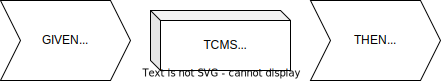
\includegraphics[scale=0.75]{images/In_out_TI_ER.png}
    \caption{Test Inputs and Expected Results}
    \label{fig:ti_er}
\end{figure}

Generated tests shall follow the the MCDC (Modified Condition/Decision Coverage) coverage criteria. MCDC is used in critical software development to ensure adequate testing. Essentialy, it states that every condition in a decision should independently affect the outcome of a decision and every decision and condition should take every possible outcome. MCDC is very similar to Active clause coverage regarding Logic Coverage \cite{intro_sw_testing}.
Meaning that, in the context of these works every predicate clause shall independently affect the outcome of this same predicate and for each clause and predicate every possible outcome is exercised.\\

It is important to mention that this requirement compiler supports predicate clauses separated by \textbf{AND} boolean operators. The reason being that the manufacturer prohibits the use of \textbf{OR} operators on system requirements by stating the following: \textit{"Multiple pre-conditions shall be linked only by AND, i.e. OR pre-conditions are forbidden."} on document \cite{tcms_req_guidelines}.\\

The use of \textit{Sesnando} on a different manufacturer project where Requirements with multiple boolean logic operator are used, require further developments on \textit{Sesnando} tool. This approach might include the reduction and simplification of the input logical expression and the application of a newly developed algorithm. These techniques have already been explored by this Github user (armin-montigny) \cite{armin-montigny_evaluation_2022}. However, \textbf{OR} operators are implicitly present on \textit{for at least} quantifiers as it will be shown further.\\

Considering the presented constrains, the outcome of a predicate is given by the Equation \ref{eq:eq1}.

\begin{equation}
    \text{Predicate Outcome} = \text{Clause1} \circ \text{Clause2} \circ \text{ClauseN}
    \label{eq:eq1}
\end{equation}


The observation of \textit{THEN} actions or effects are accorded to \textit{GIVEN} and \textit{WHEN} predicates combined, as such, this results in a similar Equation \ref{eq:eq2}

\begin{equation}
    \text{Realised THEN effects} = \text{GIVEN Predicate} \circ \text{WHEN Predicate}
    \label{eq:eq2}
\end{equation}


Meaning that a simple requirement REQ4661 containing one \textit{GIVEN} \textbf{AND} operator and a single \textit{WHEN} clause would result in a set of tests presented on Table \ref{tab:spec_single_and}.

\begin{Verbatim}[xleftmargin=12mm, numbers=left]
REQUIREMENT(REQ446-1, function, tcmsdevice) 
{
	GIVEN <SignalIn1> is equal to true
		and <SignalIn2> is equal to true;
	WHEN <SignalIn3> is equal to true;
	THEN <SignalOut1> is set to true;
}                                 
\end{Verbatim}

\begin{table}[h]
\caption{Test Spec for single AND}
    \footnotesize
    \centering
    
    \begin{tabular}{c c c c c}
        \hline
        % --- ROW Header --- %
        \textbf{\textit{Test step}} & 
        \textbf{\textit{SignalIn1}} & 
        \textbf{\textit{SignalIn2}} & 
        \textbf{\textit{SignalIn3}} & 
        \textbf{\textit{SignalOut1}}\\ \hline  \\
        
        % --- ROW 1 --- %
        \begin{tabular}[c]{@{}c@{}} \textbf{\textit{ 1 }} \end{tabular} & 
        0 & 
        1 &
        1 &
        0 \\
        \hline \\
        
        % --- ROW 2 --- %
        \begin{tabular}[c]{@{}c@{}} \textbf{\textit{ 2 }} \end{tabular} & 
        1 &
        0 &
        1 &
        0 \\
        \hline \\
       
        % --- ROW 3 --- %
        \begin{tabular}[c]{@{}c@{}} \textbf{\textit{ 3 }} \end{tabular} & 
        1 &
        1 &
        0 &
        0 \\
        \hline \\
        
        % --- ROW 4 --- %
        \begin{tabular}[c]{@{}c@{}} \textbf{\textit{ 4 }} \end{tabular} & 
        1 &
        1 &
        1 &
        1 \\
        \hline \\
        
    \end{tabular}
    \label{tab:spec_single_and}
\end{table}


Both predicates should evaluate to true in order to verify the expected results given by \textit{THEN} predicate. In other words, SignalInX will be written to the system, whereas SignalOutX will be read from the system and compared against expected results provided on Table \ref{tab:spec_single_and}.\\

For cases where a predicate clause contains a quantifier where the AND operator is implicit (e.g. For all), in order to check whether this clause affects the predicate outcome (as per MCDC), to evaluate the negative outcome of a predicate. all the quantifier signals are set to True, and the test steps start by negating each signal one-by-one as per Equation \ref{eq:for_all}. For cases where OR operator is implicit (e.g. For at least) the reverse scenario is applied as per Equation \ref{eq:for_at_least}. This is illustrated on Table \ref{tab:dbd_test_spec}. Further details of Test Generator is presented on Section \ref{sec:method}.

\begin{equation} \label{eq:for_all}
    \text{TechnicalSignal}[i] = False \quad \forall i \in \{0, 1, 2, \dots , n-1\}
\end{equation}

\begin{equation} \label{eq:for_at_least}
    \text{TechnicalSignal}[i] = True \quad \forall i \in \{0, 1, 2, \dots , n-1\}
\end{equation}

As an example, the requirement REQ4662 verbatim contains two signals whereas the <Train speed> maps to only one technical signal and the <Dragging Brake detected> maps to four signals. The clause containing the <Train speed> evaluates to true if the speed is above 3, so value 4 is used for the cases where the clause evaluates to true, and the value 3 is used when the clause should evaluate to false.

\begin{Verbatim}[xleftmargin=12mm, numbers=left]
REQUIREMENT(REQ446-2, 2F02_Traction_Braking, CCUS)
{
	GIVEN <Train speed> is greater than 3
	    and <Dragging Brake Detected> is equal to true 
	    for at least one brake in the Unit;
	WHEN;
	// Juridical Recording Unit
	THEN <JRU Dragging Brake Detected> is set to true;
}
\end{Verbatim}


Whereas, after the signal translation process, \textit{Sesnando} should retrieve multiple signals as many as there are brakes in the train unit. For simplicity and readability purposes, it will be assumed that Signal Manager returned four signals related to brakes on the train to the test generator. As it will be seen, the test specification will expand to a bigger test matrix. On the Equation \ref{eq:big_matrix}, O1 represents the output signal <JRU Dragging Brake Detected>, \textbf{m} represents the test step and \textbf{n}, the number of signals related to Requirement signal (a,b).

\begin{equation} \label{eq:big_matrix}
\text{O1} = 
Train Speed \circ Drag. Brake Det. = 
( b_i \cdot a_{ij}) = 
\begin{pmatrix} 
b_{1} \cdot  a_{11} & \cdots & a_{1n} \\
\vdots & \ddots & \vdots \\ 
 b_{m} \cdot  a_{m1} & \cdots & a_{mn} 
\end{pmatrix}
\end{equation}


So that, REQ446-2 would result in the test Table \ref{tab:dbd_test_spec}. Where Bk(x) represents each brake and TS representing the train speed technical signals. The expected result (JRU Dragging Brake Detected) for each test case is represented by JRU DBkDet.

\begin{table}[h]
\caption{Test Spec Dragging Brake Detected}
    \footnotesize
    \centering
    
    \begin{tabular}{c c c c c c c}
        \hline
        % --- ROW Header --- %
        \textbf{\textit{Test step}} & 
        \textbf{\textit{TS}} & 
        \textbf{\textit{Bk1}} & 
        \textbf{\textit{Bk2}} & 
        \textbf{\textit{Bk3}} & 
        \textbf{\textit{Bk4}} & 
        \textbf{\textit{JRU DBkDet}}\\ \hline  \\
        
        % --- ROW 1 --- %
        \begin{tabular}[c]{@{}c@{}} \textbf{\textit{ 1 }} \end{tabular} & 
        4 & 
        0 &
        0 &
        0 &
        0 &
        0 \\
        \hline \\
        
        % --- ROW 2 --- %
        \begin{tabular}[c]{@{}c@{}} \textbf{\textit{ 2 }} \end{tabular} & 
        3 &
        1 &
        0 &
        0 &
        0 &
        0 \\
        \hline \\
       
        % --- ROW 3 --- %
        \begin{tabular}[c]{@{}c@{}} \textbf{\textit{ 3 }} \end{tabular} & 
        4 &
        1 &
        0 &
        0 &
        0 &
        1 \\
        \hline \\
        
        % --- ROW 4 --- %
        \begin{tabular}[c]{@{}c@{}} \textbf{\textit{ 4 }} \end{tabular} & 
        4 &
        0 &
        1 &
        0 &
        0 &
        1 \\
        \hline \\
        
        % --- ROW 5 --- %
        \begin{tabular}[c]{@{}c@{}} \textbf{\textit{ 5 }} \end{tabular} & 
        4 &
        0 &
        0 &
        1 &
        0 &
        1 \\
        \hline \\
        
        % --- ROW 6 --- %
        \begin{tabular}[c]{@{}c@{}} \textbf{\textit{ 6 }} \end{tabular} & 
        4 &
        0 &
        0 &
        0 &
        1 &
        1 \\
        \hline \\
        
    \end{tabular}
    \label{tab:dbd_test_spec}
\end{table}

Table \ref{tab:dbd_test_spec}, is is the result of the logical expression:\\
$((TS > 3) \land (Bk1 \lor Bk2 \lor Bk3 \lor Bk4))$\\
It can be observed that, as per MCDC Coverage criteria, each clause takes every possible outcome, every decision (predicate) takes every possible outcome and each condition (clause) affects every possible decision outcome. This process is fully automated within the Test Generator module of \textit{Sesnando}.


\subsubsection{Signal Translation and quantifier signal attributes}
%----------------------- Signal Translation ----------------------------
\label{subsubsec:sub_signal_translation}

\textit{Sesnando} extracts every requirement signal from the input requirement and asks the Signal manager for its corresponding Technical signals. This is achieved by calling a Signal Manager API endpoint \\
(e.g., \textcolor{black}{https://<IP\_Address>:5001/api/signal/<LogicalSignal>}).\\

When a \textit{Logical signal} is not found, \textit{Sesnando} will report an error message to the user for the current requirement, as the signal must be added to the Database.

When a requirement is applied to a multiple set of components of the same type on the system (Doors, Brakes, Axles), \textit{Sesnando} looks to test these components individually (See Section \ref{subsubsec:test_cases}), when a requirement instructs to do so, this is achieved through the use of quantifiers as previously presented on Section \ref{tab:signal_mapping}.

All the train elements and attributes can be presented on an hierarchical format. Figure \ref{fig:hier_elem_attr} presents this said hierarchy and some of their attributes.

\begin{figure}[h]
    \centering
    \includegraphics[width=\textwidth]{images/hier_elems_attrs.PNG}
    \caption{Table train elements and attributes (excerpt)}
    \label{fig:hier_elem_attr}
\end{figure}

Element attributes are important during the generation of the test cases. There is a train functionality that, regarding the location of train, the Driver might not be allowed to open the doors for a given side. This behavior is presented on the following requirement verbatim.


\begin{Verbatim}[xleftmargin=12mm, numbers=left]
REQUIREMENT(REQ446-3, function, tcmsdevice) 
{
	GIVEN <Door Open Permit> is equal to true for one side;
	WHEN <Driver Desk Door Open> is equal to true 
	    for the same side;
	THEN <TCMS command door open> is set to true 
	    for the same side;
}
\end{Verbatim}

The signals on Figure \ref{fig:hier_elem_attr} are an extract from a test script related to <Door open permit>. These are used as an example to present the signal attributes.

\begin{figure}[H]
    \centering
    \includegraphics[width=\textwidth]{images/door_prmt.PNG}
    \caption{Door open permit signals}
    \label{fig:hier_elem_attr}
\end{figure}

The signal attributes from signals on Figure \ref{fig:hier_elem_attr} are presented on Figure \ref{fig:door_perm_sig_attr}, which are extracted from the project documentation (e.g. ICDs and ISLs) and are then populated on Signal manager to support the generation of tests by \textit{Sesnando}.

\begin{figure}[H]
    \centering
    \includegraphics[width=\textwidth]{images/signal_attr_dp.PNG}
    \caption{Door open permit signals attributes}
    \label{fig:door_perm_sig_attr}
\end{figure}


So that, REQ4662 would result in the test Table \ref{tab:for_the_same_test_spec}. Where DOPlft and DOPRgt represents <Door Open Permit> technical signals, DDDOLft and DDDORgt <Driver Desk Door Open> the technical signal for the Driver Door open command. The expected result (<TCMS command door open>) for each test case is represented by TCMSDOLft and TCMSDORgt.

\begin{table}[H]
\caption{Test Spec - for the same quantifier}
    \footnotesize
    \centering
    
    \begin{tabular}{c c c c c c c}
        \hline
        % --- ROW Header --- %
        \textbf{\textit{Test step}} & 
        \textbf{\textit{DOPlft}} & 
        \textbf{\textit{DOPRgt}} & 
        \textbf{\textit{DDDOLft}} & 
        \textbf{\textit{DDDORgt}} & 
        \textbf{\textit{TCMSDOLft}} & 
        \textbf{\textit{TCMSDORgt}}\\ \hline  \\
        
        % --- ROW 1 --- %
        \begin{tabular}[c]{@{}c@{}} \textbf{\textit{ 1 }} \end{tabular} & 
        0 & 
        1 &
        0 &
        0 &
        0 &
        0 \\
        \hline \\
        
        % --- ROW 2 --- %
        \begin{tabular}[c]{@{}c@{}} \textbf{\textit{ 2 }} \end{tabular} & 
        1 &
        0 &
        0 &
        0 &
        0 &
        0 \\
        \hline \\
       
        % --- ROW 3 --- %
        \begin{tabular}[c]{@{}c@{}} \textbf{\textit{ 3 }} \end{tabular} & 
        1 &
        1 &
        0 &
        0 &
        1 &
        0 \\
        \hline \\
        
        % --- ROW 4 --- %
        \begin{tabular}[c]{@{}c@{}} \textbf{\textit{ 4 }} \end{tabular} & 
        0 &
        0 &
        0 &
        1 &
        0 &
        0 \\
        \hline \\
        
        % --- ROW 5 --- %
        \begin{tabular}[c]{@{}c@{}} \textbf{\textit{ 5 }} \end{tabular} & 
        0 &
        0 &
        1 &
        0 &
        0 &
        0 \\
        \hline \\
        
        % --- ROW 6 --- %
        \begin{tabular}[c]{@{}c@{}} \textbf{\textit{ 6 }} \end{tabular} & 
        0 &
        0 &
        1 &
        1 &
        0 &
        1 \\
        \hline \\
        
    \end{tabular}
    \label{tab:for_the_same_test_spec}
\end{table}


\textit{Sesnando} internally divides the testing for both sides into two test cases (1-3,4-6), for left and right. In other words, for as many sides there are on the train.
The quantifier \textit{for the same} is under a conceptual phase and hasn't been fully implemented yet.


\subsection{Signal Manager}
%----------------------- Signal Manager ----------------------------
\label{subsec:signal_manager}

Ideally, \textit{Signal Manager} should run on a remote server where the testing information is centralized. The main benefits of this approach is that every tester, developer or project stake-holder can contribute to develop a solid knowledge base to sustain the test generation from \textit{Sesnando Compiler} instance.\\

\textit{Signal Manager} can be accessed trough a Web Interface running on port 5001. From there, the user is able to edit Technical signals (Software signals) which can be mapped to the corresponding Logical Signals (Requirement Signals) as well as add relevant data like attributes and states. See (Fig. \ref{fig:signal_manager_pibs})

\begin{figure}[H]
    \centering
    \includegraphics[width=\textwidth]{images/signal_manager_signals_pibs.PNG}
    \caption{Signal Manager PIBS Signal Mapping example}
    \label{fig:signal_manager_pibs}
\end{figure}

The Figure \ref{fig:signal_manager_pibs} is an excerpt from the \textit{Signal Manager} interface. It can be seen that a set of technical signals are mapped to a Logical Signal trough an Id value. A Technical signal might accept several attributes, e.g., a door \textit{Side} or Car location within the train or a state, e.g., Open, Released, Closed, that might be represented through an integer number, this is defined from the original requirement, e.g., "Given <Door status> is equal to Released".


\subsection{Test Designer}
%----------------------- Test Designer ----------------------------
\label{subsec:test_designer}

The main goal of \textit{Test Designer} is to display the generated test specification to the user. The user is able to modify it as intended and from there, generate a test script. This interface is presented on the next image (Fig. \ref{fig:test_designer_interface}).

\begin{figure}[H]
    \centering
    \includegraphics[width=\textwidth]{images/test_designer.PNG}
    \caption{Test Designer Interface}
    \label{fig:test_designer_interface}
\end{figure}

The above image (Fig. \ref{fig:test_designer_interface}) is the result of a scalar requirement signal evaluating to int value "1" combined with an \textit{AND} operator to a quantifier requirement signal. Tests are executed from top to bottom.
The first row of the table corresponds to the software technical signal, the second row defines the direction of the signal as:

\begin{itemize}
    \item in\_write - The value to be \textit{forced} on the corresponding technical signal.
    \item out\_write - The expected results according the test inputs from the left input columns.
\end{itemize}

Test designer test tables are representations of test specifications presented on Section \ref{subsec:test_generation}.


\subsubsection{Generated Artifacts and test execution}
%----------------------- Generated Artifacts ----------------------------
\label{subsubsec:generated_artifacts}

After visualising and reviewing the test specification on the test designer, the tester will be able to export it into a test script compatible with the test execution tool. This feature can be located by navigating to "File -> Export to test script". At this moment \textit{Sesnando} only supports one script type but it is intended that the user interface could be extended to support multiple script types as needed.\\
With this, it is intended to demonstrate a complete end-to-end lifecycle, from requirements to test execution. Next, is a tool that allows the observation of the internal states of a simulated train in operation (Fig. \ref{fig:test_environment})

\begin{figure}[H]
    \centering
    \includegraphics[width=\textwidth]{images/test_environment.png}
    \caption{Test Environment}
    \label{fig:test_environment}
\end{figure}

The validation facility (which might be in a form of Test Rack or a local testers' computer, Section \ref{sec:current_procedures}) loads the script generated from \textit{Sesnando}. On a simple operation, the signal values start to be set on the software to produce the desire outcomes. The real-time value of every software signal through the test time-span can be observed on the multi-chart present on the software tool (Fig. \ref{fig:test_environment}). This also demonstrates that \textit{Sesnando} is able to generate test scripts from the input requirements that are compatible with the presented test environment.




